\documentclass{article}
\usepackage[utf8]{inputenc}
\usepackage{multicol}
\usepackage{graphicx}
\usepackage[round]{natbib}
\usepackage{hyperref}
\usepackage{amsmath}
\usepackage{framed}
\usepackage{palatino}
\usepackage[absolute]{textpos}
\usepackage{xcolor}
\usepackage{setspace}
\onehalfspacing

\begin{document}
\begin{titlepage}
\def\coverborderleft{30mm}
\definecolor{UniversitaetFarbe}{RGB}{0,101,189}

\begin{textblock*}{\textwidth}(\coverborderleft, 2cm)
\noindent
\textcolor{UniversitaetFarbe} {
  \fontsize{9}{11}\selectfont
  \sffamily Master of Science in Transportation Systems\\
  \sffamily Ingenieurfakultät Bau Geo Umwelt\\
  \sffamily Technische Universität München}
\end{textblock*}

\begin{textblock*}{19mm}[1,0](19cm, 2cm)
  
\includegraphics{TUM_blau.pdf}
\end{textblock*}

\begin{textblock*}{\paperwidth}(\coverborderleft, 6cm)
\raggedright
  \sffamily \huge{The Feedback Loop of Cycling and Walking} \\
  \sffamily \Large{David Bailey (david.bailey@tum.de) | 03682683}\\
  \sffamily \large{February 2017}\\
\end{textblock*}
~\\
\end{titlepage}

\section*{Abstract}
\subsection*{Objective}
This paper proposes that the low rates of cycling and walking for transportation in the United States are the result of feedback loop. This loop, caused by nonexistent and poor quality infrastructure, results in high fatality and injury rates for cyclists and pedestrians and low rates of cycling. Furthermore, low rates of cycling and walking promote auto-centric infrastructure that is unsafe and uncomfortable for cycling and walking.
\subsection*{Methods}
This research utilized a combination of literature review from scientific journals and data analysis from government sources. 
\subsection*{Results}
The feedback loop is examined step-by-step. Studies document the lack of quality cycling and walking infrastructure, high rates of fatalities and injuries among cyclists and pedestrians, low rates and cycling and walking, and the promotion of auto-centric infrastructure.
\subsection*{Discussion}
The only way to reduce fatalities and injuries and increase rates of walking and cycling is through the construction of cycling and pedestrian infrastructure such as cycle lanes, open streets events, and bike share systems. Additionally, policy changes away from single-use zoning towards more diverse urban neighborhoods improve pedestrian activity. Feedback loops can also work to promote modes such as automobiles in the United States and walking, cycling, and public transportation in some European cities.
\subsection*{Conclusions}
Cities that wish to lower rates of cyclist and pedestrian injuries and increase rates of cycling and walking must do so by building cycling and pedestrian infrastructure.
\section*{Introduction}
Across the United States, cyclists and pedestrians face high rates of fatalities and injuries \citep{fhwa2016}. Additionally, cycling and walking make up a small percentage of commuters \citep{uscb2016}. Many cities across the United States have also adopted the Swedish policy of Vision Zero to eliminate traffic fatalities and serious injuries and wish to raise rates of cycling and walking. In this paper, we investigate why rates of cycling and walking fatalities are so high and why rates of cycling and walking are so low. We propose that cycling and walking (collectively called non-motorized transportation or active transportation), as a component of the transportation system in the United States, are stuck in a feedback loop (Figure \ref{fig:feedbackloop}). In this loop infrastructure creates unsafe and uncomfortable conditions, these conditions dissuade people from cycling and walking, and consequently the resulting low percentage of cyclists and pedestrians further drives infrastructure to be unsafe and uncomfortable for cycling and walking. While specifics of the loop differ between cycling and walking, the overall system functions the same. The feedback loop has four steps:

\begin{enumerate}
    \item Cycling and pedestrian infrastructure in the United States is often nonexistent, and the infrastructure that does exist is often poor quality compared to international leaders in cycling and walking.
    \item As a result of this infrastructure, those who do choose to cycle or walk face unsafe and uncomfortable conditions. Fatality and injury rates for cyclists and pedestrians are high compared to both other transportation modes in the United States and to fatality and injury rates of international leaders in cycling and walking.
    \item Because of the actual and perceived unsafe and unconformable conditions for cyclists and pedestrians in the United States, few people choose cycling or walking as their primary mode of transportation.
    \item Because of the low rate of cycling and walking in the United States, transportation planners and engineers do not consider the needs of cyclists and pedestrians when designing new infrastructure or maintaining old infrastructure. Additionally, the collective voice of cyclists and pedestrians is small compared to motorists and improvements to cycling and pedestrian infrastructure are often dismissed by political leaders who seek to build voter support. Transportation infrastructure continues to primarily support motorists with little regard for the safety or comfort of cyclists or pedestrians.
\end{enumerate}

\begin{figure}
    \centering
    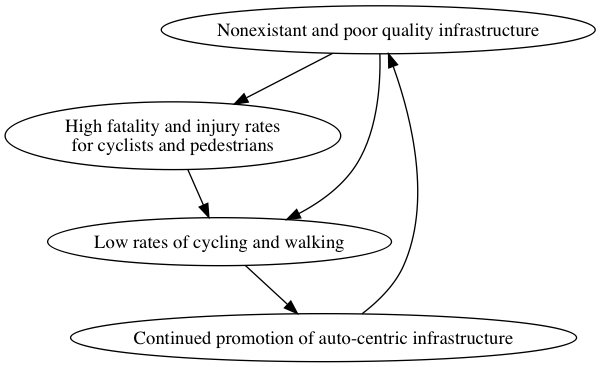
\includegraphics[width=11cm]{feedbackloop}
    \caption{The Feedback Loop of Cycling and Walking}
    \label{fig:feedbackloop}
\end{figure}

\section*{Methods}
This research utilized a combination of literature review from scientific journals and data analysis from government sources. For the data analysis portion, we compared the rates of commuting by different modes from United States Census Bureau American Community Survey 5-Year Data (2009-2015) with the rates of fatalities and serious injures from the California Statewide Integrated Traffic Records System and the United States National Highway Traffic Safety Administration Fatality Analysis Reporting System (FARS) Encyclopedia.

\section*{Results}

\subsection*{Nonexistent and poor quality infrastructure}
Different types of road designs result in different injury risks for cyclists. Major streets with parked cars tend to have the greatest injury risk for cyclists, major streets without parked cars have a lower injury risk, local streets have an even lower risk, and protected bike lanes tend to have the lowest injury risk for cyclists \citep[Page 2340]{teschke2012}. However, protected bike lanes (also called cycle tracks) are uncommon in the United States and most cyclists must cycle on major streets during some portion of their journey \citep[Page 2-3]{mekuria2012}. This condition of infrastructure has two factors: first, potential cyclists will choose a mode other than cycling for their trips as discussed later, and second those who choose to cycle are at a much greater risk of injury than cyclists in countries with high quality infrastructure such as protected bike lanes. Additionally, when cities do improve their cycling infrastructure, the rate of cycling injuries decreases \citep[Page 2173]{pedroso2016} \citep[Page 2090]{pucher2016}.

A similar situation exists for pedestrians where inadequate infrastructure results in greater risk to pedestrians \citep{who2013}. Additionally, pedestrians must often confront long distances, missing or inadequate sidewalks, sidewalks close to loud and busy streets, hot conditions with no shade or cold conditions, and an abundance of parking lots instead of ground floor retail or landscaping.

Bicycle facilities are categorized by several different methods. Bicycle Level of Service and Bicycle Compatibility Index rely on complex formulas to derive a ranked rating from A to F. However, these ratings are often inadequate and do not correspond the the abilities of cyclists \citep[Page 13]{mekuria2012}. The Levels of Traffic Stress (LTS) provide a mapping between cycling infrastructure and the suitability for different types of cyclists \citep[Page 13-14]{mekuria2012}.

\begin{table}[h]
  \centering
\begin{tabular}{ l l }
    Level & Description \\
    \hline
    LTS 1 & Suitable for almost all cyclists \\
    LTS 2 & Suitable for most adult cyclists \\
    LTS 3 & Suitable for current cyclists \\
    LTS 4 & Beyond LTS 3 \\
\end{tabular}
    \caption{Levels of Traffic Stress (LTS) \citep{mekuria2012}}
    \label{table:lts}
\end{table}

LTS incorporates the presence of bike lanes, number of lanes, street width, speed limits or prevailing speeds and rarity of bike lane blockage to determine the level of stress. Additionally, LTS incorporates the design of intersection approaches and crossings \citep[Page 17-21]{mekuria2012}. These criteria have been proven to be stressors for cyclists by measuring galvanic skin response, a common physiological indicator of stress \citep{caviedes2016} \citep{liu2016}. When evaluating a road for LTS, the segment with the highest (worst) level of stress determines the level for the whole road. Similarly, when evaluating a route for LTS, the route with the highest (worst) level of stress determines the level of stress for the whole route. Consequently, while there can be many areas of low stress roads, these areas are often disconnected from each other as unconnected islands of low stress. Also, there is a limit to how far a potential cyclist will go to access a low stress route.

Cyclists (and drivers) prefer buffered bike lanes and protected bike lanes over streets with unprotected bike lanes or no cycling facilities \citep[Page 6]{monsere2012} \citep[Page 10]{mcneil2015}. Pedestrians also prefer walking on streets with protected bike lanes. Additionally, women's preferences for infrastructure differs from men \citep[Page 2174]{pedroso2016}, and women are much more likely to prefer off-road cycle paths over other types of facilities \citep[Page 5]{monsere2012} \citep[Page 57]{garrard2008}. In countries with high rates of cycling, women make up about 50\% of cyclists. In countries with low rates of cycling, women make up less than 25\% of cyclists.

Pedestrians face similarly poor conditions for walking. The focus of traffic engineering in the United States has been concentrated on speeding up cars by widening lanes and roads and enlarging turning radii \citep[Page 14]{mccann2000}. Consequently, increases in speed result in higher pedestrian fatalities and injuries. Little focus is put on traffic calming or creating quality infrastructure for pedestrians.

\subsection*{High fatality and injury rates for cyclists and pedestrians}
Although less than 4\% of Californians commuted to work primarily by walking (2.7\%) or cycling (1.1\%) in 2015 \citep{uscb2016} (Figure \ref{fig:commutersbymode}), almost 25\% of Californians killed or seriously injured in traffic collisions in the same year were walking (17.3\%) or cycling (7.3\%) \citep{chp} (Figure \ref{fig:victimsbymode}). These tragic circumstances are consistent across recent years and present throughout the United States \citep{nhtsa}.

\begin{figure}[p]
    \centering
    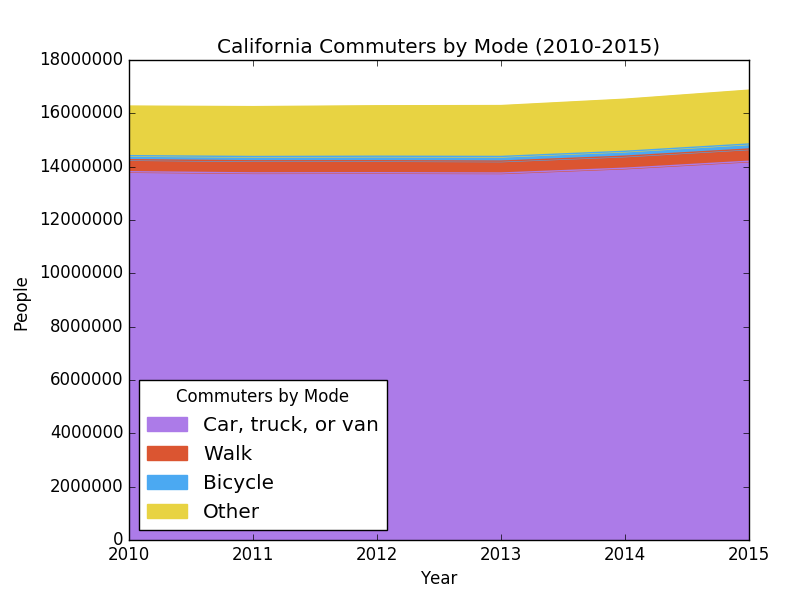
\includegraphics[width=11cm]{commutersbymode}
    \caption{California Commuters by Mode (2010-2015)}
    \label{fig:commutersbymode}
\end{figure}

\begin{figure}[p]
    \centering
    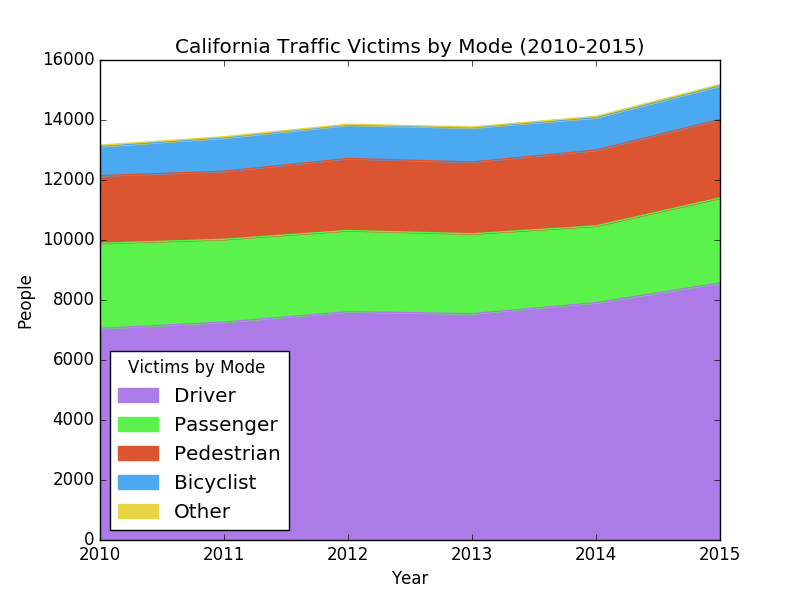
\includegraphics[width=11cm]{victimsbymode}
    \caption{California Traffic Victims by Mode (2010-2015)}
    \label{fig:victimsbymode}
\end{figure}

From 2002 to 2005, cyclists in the United States experienced much higher fatality and injury rates than cyclists in the Netherlands, Germany, and Denmark \citep[Page 1512]{pucher2003}. Cyclists in the United States were over 5 times more likely to be killed per kilometer cycled than those in the Netherlands and 3-4 times more likely to be killed than cyclists in Denmark and Germany \citep[Page 12]{pucher2008}. Additionally, fatality rates in the Netherlands, Germany, and Denmark have all fallen much more in the past two decades than in the United States \citep[Page 283]{buehler2017}.

 \begin{figure}
    \centering
    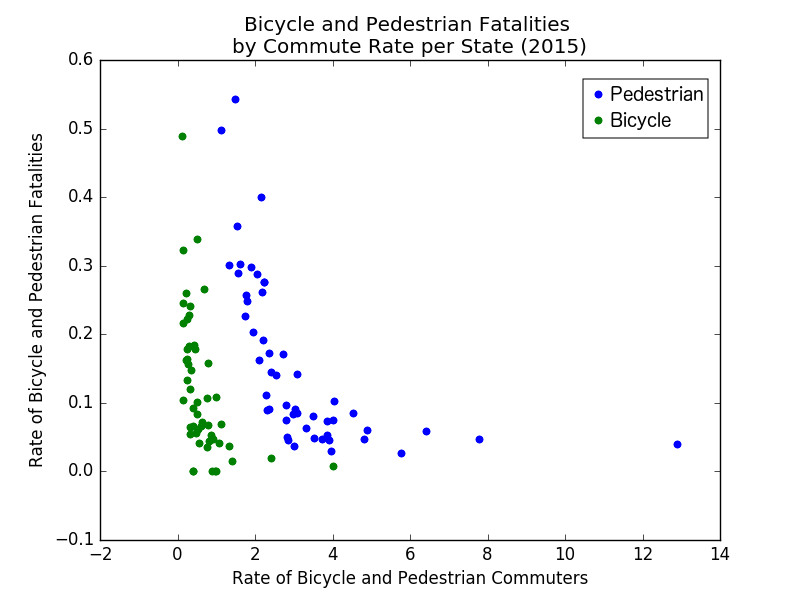
\includegraphics[width=11cm]{usrates}
    \caption{Bicycle and Pedestrian Fatalities by Commute Rate per State (2015)}
    \label{fig:usrates}
\end{figure}

Cyclists and pedestrians tend to experience lower rates of fatalities and injuries in areas with more cyclists and pedestrians \citep[Page 208]{jacobsen2003}. This holds for United States bicycle and pedestrian commuters in 2015 (Figure \ref{fig:usrates}) \citep{uscb2016} \citep{nhtsa}. States with the highest percentage of bicycle commuters, Washington DC (4.0\%) and Oregon (2.4\%), are in the top 10 safest states according to cyclist fatality risk. Similarly, states with the highest percentage of pedestrian commuters, Washington DC (12.9\%), Alaska (7.8\%), and New York (6.4\%), are in the top 15 safest states according to pedestrian fatality risk. The same correlations hold true for the states with the greatest risk to cyclists and pedestrians. Additionally, the same correlations exist for county-level data for the state of California where Yolo and San Francisco counties have the two highest rates of cycling and some of the lowest rates of fatalities and severe injuries \citep{uscb2016} \citep{chp}.

Jacobsen proposes this correlation could be caused by a change in driver behavior in areas with more cyclists and pedestrians \citep[Page 208]{jacobsen2003}. These drivers become more cautious and aware of cyclists and pedestrians when they are around them more often. However, correlation does not imply causation. Instead of assuming driver behavior to be dependent on the presence of cyclists and pedestrians, perhaps, driver, cyclist, and pedestrian behavior are all dependent on the surrounding infrastructure and to a lesser extent traffic law enforcement and traffic education in the area. In other words, cyclists and pedestrians tend to cycle and walk more in areas where they are and feel safer. This idea fits logically with the theory of the feedback loop of cycling and walking \citep[Page 8]{teschke2015}.
 
Improvements in cycling infrastructure cause both increased rates of cycling and decreased rates of cycling crashes, severe injuries, and fatalities \citep{pucher2016}. These improvements should take the form of separating bicycles and motor vehicles on high-speed roads and modifying lanes and intersections to decrease the severity of potential collisions \citep{cushing2016}. Additionally, infrastructure improvements should be supported by investments in education, enforcement, and cycling encouragement activities. However, without infrastructure improvements, these secondary measures will not be able to reduce traffic fatalities and serious injuries by themselves.

\subsection*{Low rates of cycling and walking}
As shown in (Figure \ref{fig:usrates}), the United States has relatively low rates of cycling and walking. Only in Washington DC do cyclists and pedestrians comprise more than 10\% of all commuters. With such poor infrastructure and high fatality and injury rates, this is not surprising. Safety is the number one reason more people do not bicycle \citep[Page 1]{geller2006}. 

Potential cyclists can be generally divided into 4 categories based on their willingness to ride provided different levels of infrastructure: Strong \& Fearless, Enthused \& Confident, Interested but Concerned, and No Way No How (Table \ref{table:fourtypes}) \citep[Page 3]{geller2006} \citep[Page 6-7]{dill2012}.

\begin{table}[h]
  \centering
\begin{tabular}{ l l r }
    & & Percent of \\
    Type & Description & Population \\
  \hline
    Strong \& Fearless & Comfortable on any street & \textless1\% \\
    Enthused \& Confident & Comfortable with bike lanes & 7\% \\
    Interested but Concerned & Comfortable with bike paths & 60\% \\
    No Way No How & Physically unable or not interested & 33\% \\
\end{tabular}
    \caption{The Four Types of Cyclists \citep{geller2006}}
    \label{table:fourtypes}
\end{table}

In the United States, only the Strong \& Fearless and those without another choice commute by cycling. However, countries with better cycling infrastructure have much higher rates of cycling. For example, many cities in The Netherlands, Denmark, and Germany have cycling mode shares above 25\% or more \citep[Page 45]{pucher2008}. These countries also have walking rates between 16\% and 24\% \citep[Page 35]{buehler2012}. The vast majority (98\%+) of potential cyclists, Enthused \& Confident and Interested but Concerned, will only cycle when there is quality bicycle infrastructure. 

This rational travel behavior can be explained by personal transportation choices based on economics. The utility of a given mode of travel for a particular trip determines the likelihood a traveler will choose that mode against other available modes. This utility can be approximated by adding the monetary cost (vehicle ownership and operation cost, transit fares, parking, etc.), travel time, and comfort of the mode for the trip \citep{litman2016}. Comfort is a term which includes health and safety of the traveler.
\begin{equation}
  utility_{mode} = monetary\_cost_{mode} + travel\_time_{mode} + comfort_{mode}
\end{equation}
For cycling and walking trips, the monetary cost of an individual, day-to-day trip is negligible. This simplifies the utility of these trips to travel time and comfort.
\begin{equation}
  utility_{cycling/walking} = travel\_time_{cycling/walking} + comfort_{cycling/walking}
\end{equation}
Therefore a traveler with a car available will choose the car when the travel time and comfort of a car trip is greater than that of cycling or walking.
\begin{align}
  & monetary\_cost_{car} + travel\_time_{car} + comfort_{car} > \nonumber \\
  & travel\_time_{cycling/walking} + comfort_{cycling/walking}
\end{align}
This equation helps explain the choices travelers make regarding driving, cycling, and walking. In the United States, destinations are often so far away that the travel time spent walking is so large that people choose the car. There is simply not enough time in a person's one hour per day travel time budged for them to walk \citep[Page 36]{zahavi1974}. Similarly, reaching even nearby destinations by cycling is often so unsafe and uncomfortable that people choose the car. This is true even during heavy traffic congestion where the travel time for a cycling trip may be less than the travel time for a car trip. Additionally, cyclists and pedestrians have the highest commute well-being, a measure that includes arrival time confidence, stress, boredom/enthusiasm, excitement, enjoyment, ease of trip, and comparison to usual \citep[Page 4-5]{smith2016}. However, the vast majority of Americans still choose the car.

\subsection*{Continued promotion of auto-centric infrastructure}
The transportation system in the United States is primarily built for the car \citep[Page 1]{sciara2003}.
The primary mode of transportation in the United States is the car. 95.5\% of workers 16 years or older live in a household with at least one car. However, this rate is lower in cities and falls to 53.7\% in New York City \citep{uscb2016}.

Transportation funding levels for cycling and pedestrian projects in the United States is hard to determine. This is due to the multilevel system of transportation funding in the United States (federal, state, county, local) and because many cycling and pedestrian improvements are part of larger projects. However, in 2014, of the funds administrated by the Federal Highway Association, \$79,429,000 of \$52,436,222,000, or 0.15\% were classified in the Transportation Alternative category which includes cycling and walking \citep{fhwaohpi2014}. The remaining 99.85\% of projects were focused on improving conditions for cars and trucks. The California Department of Transportation estimated that California alone will need to spend \$4 billion on cycling infrastructure and \$60 billion on pedestrian infrastructure to meet its goals by 2040, but since 2014 the state has only spent \$1 billion, or approximately 1\% of annual transportation funding  \citep[Page 13, 86]{caltrans2017}.

\section*{Discussion}
This feedback loop of walking and cycling is relatively stable and has existed in the United States for decades. In countries that currently have excellent cycling and pedestrian infrastructure and a high rate of cycling and walking a corresponding feedback loop exists that is essentially the inverse of the loop described above: excellent infrastructure promotes cycling and walking over other modes, people respond by cycling and walking at high rates, and consequently the government responds by continuing to build quality cycling and pedestrian infrastructure. Interestingly, this type of feedback loop also exists in the United States for motorists: auto-centric infrastructure supports driving, people respond by driving, the government responds by building auto-centric infrastructure. All of these choices exist within the context of safety and comfort of the  travelers and their chosen modes. Another feedback loop exists for public transportation in most parts of the United States that keeps rates of public transportation low.

As mentioned in the introduction, many cities across the United States wish to both reduce their traffic fatalities and increase the mode share of cycling and walking. To accomplish either and both of these goals requires changing one of the stages of the feedback loop of cycling and walking. However, the only stages that can be changed independently of the loop are the promotion of auto-centric infrastructure and the condition of cycling and walking infrastructure. In the Swedish policy of Vision Zero currently being adopted by many United States cities, traffic fatalities and serious injuries are  not accepted as "accidents" or a natural consequence of travel, but rather are considered to be the results of poor road designs that do not allow for the inevitable mistakes of road users \citep[Page 2178]{cushing2016}.

Building cycling infrastructure increases bicycle commuting \citep[Page 7]{dill2003}. People respond to new cycling infrastructure, in particular the addition of protected bike lanes or the addition of any bike infrastructure where there previously was none, by cycling more \citep[Page 2174]{pedroso2016} \citep[Page 63]{monsere2014}. New cycling infrastructure also shifts people from car trips to bicycle trips \citep[Page 67]{monsere2014} most often because of the increased comfort level of the new facility \citep[Page 7-9]{mitra2016}. New cycling infrastructure increases the perception of safety by cyclists, and to a lesser extent drivers and pedestrians \citep[Page 105]{monsere2014}.

Potential cyclists in the Enthused and Confident category and especially the Interested but Concerned category state they would be more likely to ride if bicycles and motor vehicles were physically separated. Also, women are more likely to cycle more when protected bike lanes are built \citep[Page 128]{monsere2014}.

Bicycle share programs can also cause potential cyclists to shift from driving to bicycle use
\citep[Page S114]{pucher2010}. These programs are also often implemented along with the addition of bicycle lanes and are located in areas with relatively greater amounts of cycling infrastructure.

Open streets events are another way to reach Enthused \& Confident and Interested but Concerned potential cyclists. One CicLAvia event in April 2014 attracted between 37,700 and 53,950 participants, cyclists and pedestrians, and had a net cost of \$339,700 \citep[Page 30]{cohen2016}. Also, although only 8.5\% of participants usually get around Los Angeles by cycling and 2.1\% get around by walking, 29\% traveled to CicLAvia by bicycle and 5.6\% traveled by walking \citep[Page 29]{cohen2016}. Open streets events appear to be a relatively inexpensive way to motivate people to cycle and walk by providing a safe and comfortable place for them to cycle and walk. However, it is unknown if this has any impact on commute or day-to-day travel behavior.

There are many other types of cycling infrastructure that can improve safety and increase rates of cycling, \citep{pucher2010} and there is a lot the United States can learn from other countries \citep{fhwa2016}. Lugo also introduces the concept of human infrastructure where people can act as cycling infrastructure, both good and bad.
\begin{framed}
\noindent Human infrastructure works positively and negatively for cycling. That is, human infrastructure in the form of group rides, social networks of activists, and the presence of bike commuters during rush hour encourages cycling. Human infrastructure in the form of honking, yelling, and other aggressive motorist behaviors discourage cycling. --Adonia E. Lugo \citep[Page 206]{lugo2013}
\end{framed}

Transportation infrastructure can also be improved for pedestrians. Traffic lights are most often timed to move as many vehicles as quickly as possible. Re-timing lights to have shorter cycles and respond quicker to the presence of pedestrians reduces pedestrian travel time, often at little expense to drivers. Creating an exclusive pedestrian phase (otherwise known as a pedestrian scramble or Barns Dance) or implementing a leading pedestrian interval can improve pedestrian safety \citep[Page 10-12]{kothuri2017}. Additionally, lowering speeds reduces the probability a crash is fatal for a cyclist or a pedestrian. Even small reductions in speed can cause higher rates of survivability \citep[Page 151]{kroyer2014}.

Most of the concerns around building new cycling and walking infrastructure center around customer parking and commercial unloading. Cyclists and pedestrians spend around the same as drivers per month at restaurants, drinking places, and convenience stores. Cyclists and pedestrians sometimes spend less per trip, but tend to make more trips overall per month compared with drivers. However, at supermarkets, cyclists and pedestrians spend less per month \citep[Page 24-26]{clifton2013}.

While improving conditions for cyclists and pedestrians, it is important to remember that the decision to cycle or walk instead of driving must be voluntary from the point of view of the traveler. We should not introduce measures to force people to cycle and walk, and doing so without first building safe infrastructure for cycling and walking would be reckless and dangerous.

Last, successful programs must continuously evaluate themselves and their progress towards their goals. They must hold themselves accountable and recognize what works and what doesn't work. They must be willing to act and make change.

\section*{Conclusion}
The current high rates of cycling and walking fatalities and injuries and low rates of cycling and walking in the United States are caused by a lack of quality cycling and walking infrastructure. This situation makes the car the most attractive mode of transportation for most people which consequently emphases the construction of new auto-centric infrastructure. It is possible to break this feedback loop by building safer and more comfortable cycling and walking infrastructure. Cities that wish to lower their rates of traffic fatalities must build new infrastructure to meet these goals.
\bibliographystyle{plainnat}
\bibliography{references}
\end{document}

\iffalse
\begin{table}[h]
  \centering
\begin{tabular}{ l r }
  \multicolumn{2}{ c }{California Traffic Victims by Mode (2015)} \\
  \hline
    Driver & 56.5\% \\
    Passenger & 18.6\% \\
    Pedestrian & 17.3\% \\
    Bicyclist & 7.4\% \\
    Other & 0.3\% \\
\end{tabular}
\end{table}

\begin{table}[h]
  \centering
\begin{tabular}{ l r }
  \multicolumn{2}{ c }{California Commuters by Mode (2015)} \\
  \hline
    Car, truck, or van & 84.2\% \\
    Walk & 2.7\% \\
    Bicycle & 1.1\% \\
    Other & 12.0\% \\
\end{tabular}
\end{table}
\fi